\section{Experiment}
In this section, we first introduce the human-annotated datasets and baseline evaluation metrics.
Then we will show the results of our proposed SDC and SDC*,
and analyze the effectiveness of semantic distribution correlation and compression ratio used in summarization evaluation.

\subsection{Datasets}
In this experiment, we use 2 summarization evaluation datasets, which consist of source documents, summaries generated by different models and human-annotated scores on summaries.

\textbf{CNN/Daily Mail} (CNNDM)
~\cite{summeval} is a single document summarization dataset, which consists of 100 documents from the CNN/DailyMail dataset, each paired with 16 summaries generated by different systems
~\footnote{https://github.com/Yale-LILY/SummEval}.
Each summary was scored by 3
experts under four aspects: 
coherence, consistency,
fluency, and relevance.

\textbf{TAC 2010} (TAC)
~\footnote{https://tac.nist.gov/data/past/2010/Summ10.html} is a multi-document summarization dataset,
including 92 multi-documents with 43 generated summaries for each multi-document.
Each summary has one human-annotated overall score. The overall score is based on both coverage of all required aspects (Pyramid) ~\cite{pyramid} and linguistic quality (readability).

\subsection{Baselines}
\label{sec:baseline}
We take 4 reference-based evaluation metrics
and 2 reference-free evaluation metrics as baselines.

For reference-based evaluation, 
\textbf{ROUGE} family is the most popular evaluation metric in summarization, 
which evaluates the token sequence overlapping.
We use F1 scores of  ROUGE-1 ({\bf R-1}), ROUGE-2 ({\bf R-2}) and ROUGE-L ({\bf R-L}).
\textbf{BLEU}~\cite{bleu2002} focuses on precision with a brevity penalty. 
\textbf{METEOR (MET.)}~\cite{meteor2005}  allows word stems, synonyms and paraphrases matching.
\textbf{BERTScore (BERT.)}~\cite{bertscore} greedily 
maximizes the cosine similarity between token embeddings.

For reference-free evaluation, 
\textbf{BLANC (BLA.)}
~\cite{blanc} computes the accuracy of unmasking document tokens with a summary.
\textbf{Shannon (Shan.)}~\cite{shannon22} estimates the information content shared between a document and its summary.
As Shannon is the SOTA summarization evaluation metric, 
we add compression ratio to the information content of generated document with a prepended summary in the same way as Eq.\ref{eq:final}, which is called \textbf{Shannon* (Shan.*)}.



\subsection{Experimental Setup}
In our experiments~\footnote{Data and code are available at https://github.com/YizhuLiu/summeval}, we follow \citet{shannon22} to use GPT-2 small language model~\cite{GPT2} to compute the semantic distribution of text.
To evaluate the empirical performance of different summarization evaluation metrics, we correlate the metrics against the provided human judgement via \textbf{Pearson's $\gamma$}, \textbf{Spearman's $\rho$} and 
\textbf{Kendall's $\tau$} correlation coefficients~\cite{pearson,spearman,kendall}. 
The metrics with higher correlation with human evaluation scores are more effective.

As TAC is a multi-document summarization dataset,
we score the summary with each document in its multi-document set.
The averaged score of all documents is engaged as the final score of our proposed metrics.


\subsection{Results}
In this section, we 
analyze the effectiveness of our metrics using fine-grained semantic distribution correlation and introducing compression ratio.

\subsubsection{Main Results}
\begin{table*}[ht!]
	\centering
	\small
	%	\begin{tabular}{p{2em}<{\centering}p{2em}<{\centering}p{2em}<{\centering}p{2em}<{\centering}p{2em}<{\centering}p{2.6em}<{\centering}p{2.6em}<{\centering}p{2em}<{\centering}p{2em}<{\centering}p{2em}<{\centering}p{2em}<{\centering}p{2em}<{\centering}p{2em}<{\centering}}%{|p{7cm}|rl|}
	\begin{tabular}{lcccccccccccc}%{|p{7cm}|rl|}
		\hline
		\multirow{3}{*}{Metric}&\multicolumn{3}{c}{\bf Coh.}&\multicolumn{3}{c}{\bf Con.}&\multicolumn{3}{c}{\bf Flu.}&\multicolumn{3}{c}{\bf Rel.}\cr
		\cmidrule(lr){2-4} \cmidrule(lr){5-7} \cmidrule(lr){8-10} \cmidrule(lr){11-13} 
		& $\gamma$ &$\rho$ & $\tau$ & $\gamma$ &$\rho$ & $\tau$ & $\gamma$ &$\rho$ & $\tau$ & $\gamma$ &$\rho$ & $\tau$ \cr
		\hline
		R-1 & 18.15 &  34.41 & 23.33 & 61.18 & 18.53 &  10.00 &  56.44 &44.30 &37.66  &  60.89&  60.00& 46.67 \cr
		R-2 & 23.58 &  36.47 &  23.33 & 63.54& 12.94& 6.67 &  59.72&  43.56&30.96 &  63.78&  61.76& 43.33 \cr
		R-L & 12.43 & 21.47 &  11.67 & 55.41& -21.47 &  -18.33 &  50.39&  19.28& 12.55 & 55.44&  40.59&  25.00   \cr
		BLEU & 22.60 &  17.65 &  10.00& 54.39& -15.59&  -13.33&  52.81&  26.20& 17.57&  57.60&  39.12&  23.33  \cr
		MET. & 15.62&  45.59 &  26.67& 66.22& 67.35&  46.67&  57.95&  71.23 & 56.07 &  62.67 &  71.76&  50.00  \cr
		BERT. & 10.61 &15.88 &  6.67& 55.87& -7.35&  -6.67&  50.32&  27.08& 20.92 & 55.09 &  42.06 & 26.67\cr
		\hline
		BLA. & 14.93 & 12.35 & 11.67 & 62.94& 77.06 &  61.67&  55.02&  47.24& 34.31 &  46.90&  35.29 &  31.67\cr
		Shan. &  56.43 &  50.58 & 38.33& 68.36& 88.82&  71.67& 68.00 &  76.67 &  61.09&  71.62& 72.35& 58.33 \cr
		\hline
		SDC & 57.33 &  52.35 &  40.00& 69.78 & \bf 90.29&  \bf 73.33 &  69.47& 79.32 &  62.76 &  72.96 & 75.00 &  60.00 \cr
		SDC* & \bf 59.10 &  \bf 56.18&  \bf 43.33 & \bf 73.85& 90.00&  \bf 73.33 & \bf 73.47 & \bf 79.91 & \bf 64.44&  \bf 75.79& \bf 77.35 & \bf 63.33  \cr
		\hline
	\end{tabular}
	\caption{Correlation (\%) between human evaluation and various automatic metrics on CNNDM.}\label{tab:main}  
\end{table*}

\begin{table*}[th]
	\centering
	\small
	\begin{tabular}{|l|c|c|c|c|}
		\hline
		\bf Summary &\bf  Comp. $\downarrow$& \bf Shan. & \bf SDC & \bf SDC* \\
		\hline
		\makecell[l]{
			{\bf High-quality summary:} \\
			Chipotle will now be available for delivery with the Postmates app. \\ 
			Online and mobile orders will be available in 67 cities.
		}
		& 0.25& 0.20 & 0.20 & 0.32\\
		\hline
		\makecell[l]{
			{\bf Unfluent summary: }\\
			\textcolor{red}{Postmates app} will now be available for delivery with the \textcolor{red}{Chipotle}. \\ 
			Online and mobile orders will be available in 67 cities.
		}
		& 0.25& 0.18 & 0.15& 0.25\\
		\hline
		\makecell[l]{
			{\bf Irrelevant summary: }\\
			Chipotle will now be available for delivery with the Postmates app. \\ 
			\textcolor{red}{Mexican restaurant Chipolte will be available in 67 cities.
		}}
		& 0.24 & 0.20 & 0.17 &  0.28\\
		\hline
		\makecell[l]{
			{\bf Longer summary: }\\
			Mexican restaurant Chipotle has decided to tap into the 70 billion food\\ delivery market by teaming up with an app to bring burritos straight to\\ customers' doors. The fast-casual chain will work with the Postmates \\ app to begin offering delivery for online and mobile orders in 67 cities. \\
			The delivery fees for Postmates app at 5 and up.
		}
		& 0.70 & 0.62 & 0.33 & 0.31 \\
		\hline
	\end{tabular}
	\caption{Automatic evaluation on different summaries of the document in
		\figref{fig:exp}.
		To explain the effectiveness of our metrics,
		we create some bad summaries. The information in red are wrong information.}
	\label{tab:abl}
\end{table*}

\tabref{tab:main} shows that 
the correlation of our proposed SDC and SDC* against 
human evaluation in different correlation coefficients
are in the top 2 for every category of summary quality.
Compared with reference-based metrics, our metrics improve significantly in terms of consistency and relevance.
Because reference-based metrics depend on the 
quality and quantity of references.
The correlations of SDC and SDC* are similar in terms of consistency
since SDC* penalizes long summaries. 
Long summaries are more likely to express the information consistent with their source documents.
Our metrics focus on the information shared with 
document and summary. Compared with the SOTA reference-free 
metric (Shan.) measuring the
difference in information content between document 
and summary,
our metrics measure the difference in semantic distributions, which better notices the token order in the sequence (coherence and fluency) and the importance of each token (consistency and relevance) with respect to the sequence. Thus, our metrics perform better than Shan. 

To show the generalization of our proposed evaluation metrics, we compare the SOTA summarization evaluation metric (Shan.) and our proposed evaluation metrics on TAC in \tabref{tab:tac10}. 
Compared with Shan., SDC and SDC* are more consistent with human evaluation on TAC, demonstrating our proposed evaluation metrics can better evaluate generated summaries. As shown in \tabref{tab:main} and \tabref{tab:tac10}, as TAC is multi-document summarization evaluation dataset, the improvement of SDC and SDC* on TAC are less than that on CNNDM . As we compute the average of evaluation scores between the summary and each document in corresponding multiple documents, a good summary may get lower scores.
This is because that a good summary may not perfectly restore all the input multiple documents.

\begin{table}[ht]
	\centering
	\small
	\begin{tabular}{lccc}%{|p{7cm}|rl|}
		\hline
		\multirow{3}{*}{Metric}&\multicolumn{3}{c}{\bf Overall}\cr
		\cmidrule(lr){2-4}
		& $\gamma$ &$\rho$ & $\tau$ \cr
		\hline
		Shan. &  75.44 &  63.11 & 45.46 \cr
		SDC & 75.91 &  65.14 &  46.57\cr
		SDC* & \bf 75.94 &  \bf 66.36&  \bf 47.69\cr
		\hline
	\end{tabular}
	\caption{Correlation (\%) between human evaluation and automatic metrics on TAC.}\label{tab:tac10}  
\end{table}

\subsubsection{Ablation Study}
The improvement of our metrics is from {\em semantic distribution correlation}
and {\em compression ratio}. We evaluate the variants of the SOTA summarization evaluation metric (Shan.) and our proposed reference-free summarization evaluation metric (SDC*) on CNNDM.

\textbf{Semantic distribution correlation.}
Semantic distribution is a finer representation of a document,
that is, the tokens' order and tokens' weight.
The tokens' order decides the linguistic quality of a text, 
so SDC-based scores are more sensitive to the linguistic quality.
As shown in \tabref{tab:main}, SDC and SDC* perform much better than 
baselines for evaluating coherence and fluency, 
as these two evaluation directions focus on linguistic quality.
Compared with the high-quality summary, the unfluent summary and the irrelevant summary in \tabref{tab:abl} get the similar Shannon scores and lower SDC scores,
which also shows that the semantic distribution is useful.
The tokens' weight points out the important information in the document.
Although information content can represent the key content,
it cannot compare the importance among adjacent tokens,
which weakens the measure of semantic relevance.
As shown in \tabref{tab:main} and \tabref{tab:abl},
our metrics improve the evaluation on consistency, relevance and overall score.
The difference in SDC-based scores between the irrelevant summary and the high-quality summary is more significant than Shan. score.

\textbf{Compression ratio.}
To discuss the impact of compression ratio on summarization evaluation,
we introduce compression ratio into Shan. and get Shan.* (See \secref{sec:baseline}).
As shown in \figref{fig:cr}, after adding compression ratio, 
the evaluation metrics have a strengthening trend.
Meanwhile, the longer summary in \tabref{tab:abl}, which is redundant, is more likely to represent more information of the document. Thus, it is necessary to import compression ratio to the metrics only considering information coverage.

\begin{figure}[th]
	\centering
	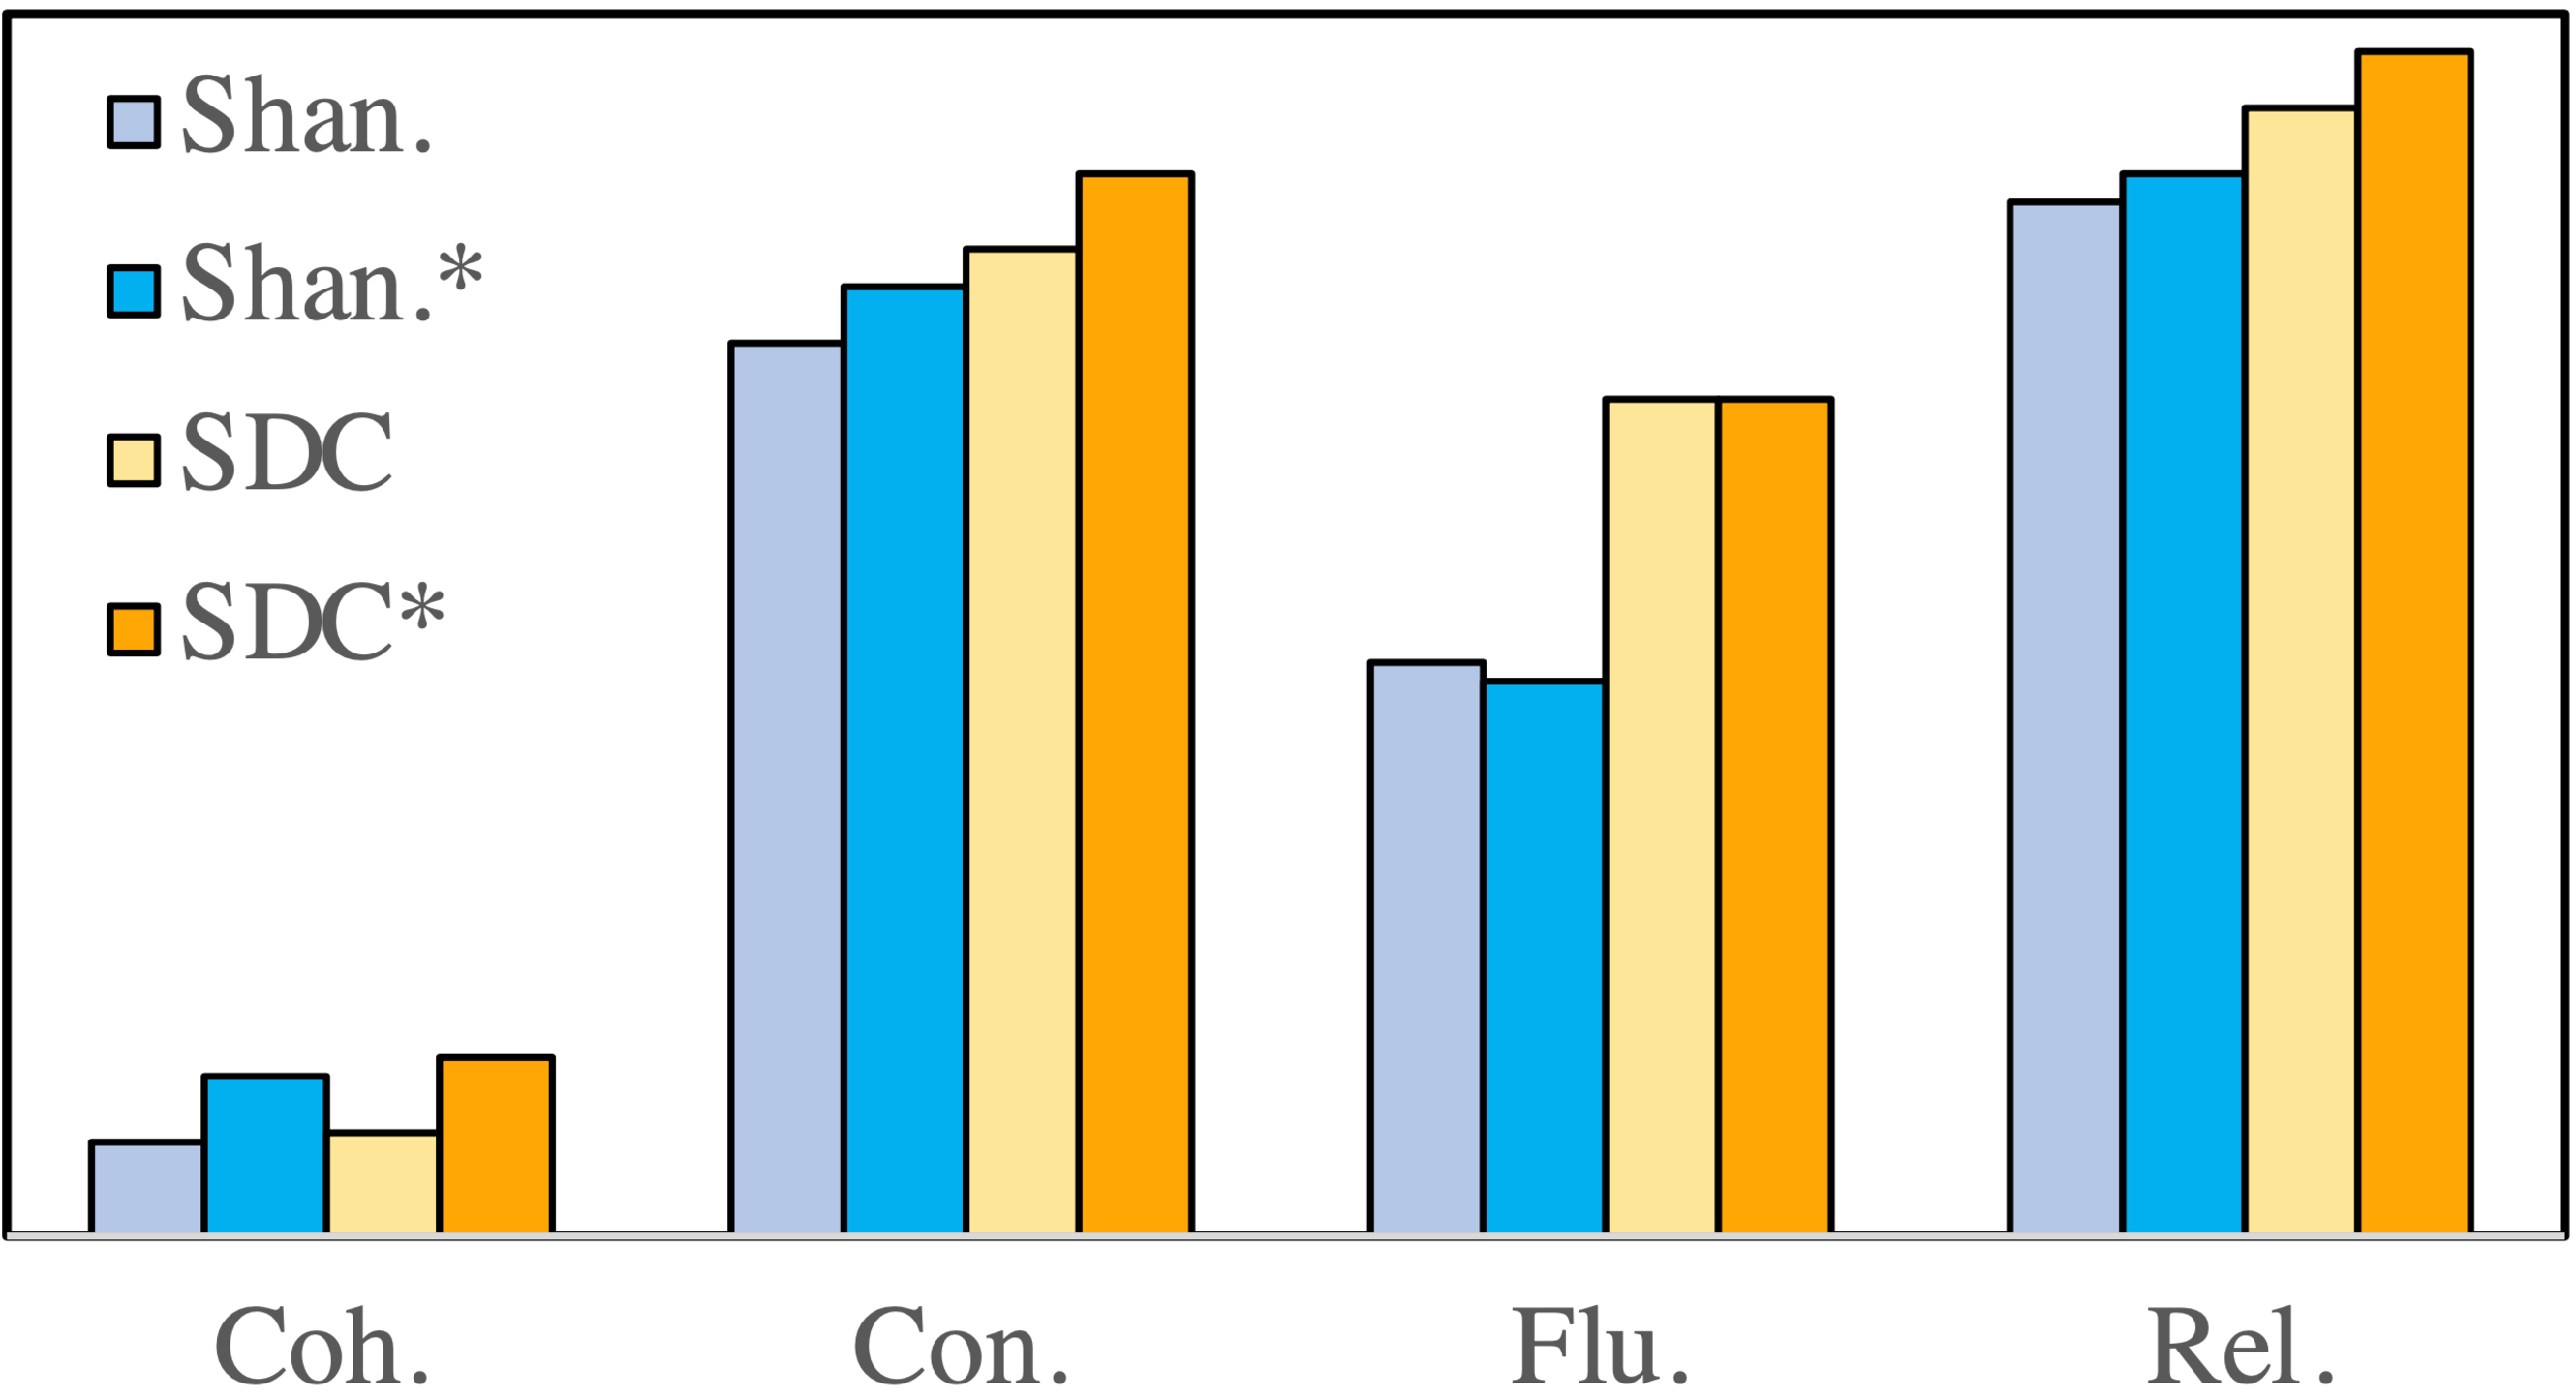
\includegraphics[width=0.65\linewidth]{comp.pdf}
	\caption{Kendall's $\tau$ correlation of evaluation metrics with and without compression ratio.}
	\label{fig:cr}
\end{figure}








